%%
% Plantilla de Memoria
% Modificación de una plantilla de Latex de Nicolas Diaz para adaptarla 
% al castellano y a las necesidades de escribir informática y matemáticas.
%
% Editada por: Mario Román
%
% License:
% CC BY-NC-SA 3.0 (http://creativecommons.org/licenses/by-nc-sa/3.0/)
%%

%%%%%%%%%%%%%%%%%%%%%
% Thin Sectioned Essay
% LaTeX Template
% Version 1.0 (3/8/13)
%
% This template has been downloaded from:
% http://www.LaTeXTemplates.com
%
% Original Author:
% Nicolas Diaz (nsdiaz@uc.cl) with extensive modifications by:
% Vel (vel@latextemplates.com)
%
% License:
% CC BY-NC-SA 3.0 (http://creativecommons.org/licenses/by-nc-sa/3.0/)
%
%%%%%%%%%%%%%%%%%%%%%

%----------------------------------------------------------------------------------------
%	PAQUETES Y CONFIGURACIÓN DEL DOCUMENTO
%----------------------------------------------------------------------------------------

%% Configuración del papel.
% microtype: Tipografía.
% mathpazo: Usa la fuente Palatino.
\documentclass[a4paper, 11pt]{article}
\usepackage[protrusion=true,expansion=true]{microtype}
\usepackage{mathpazo}

% Indentación de párrafos para Palatino
\setlength{\parindent}{0pt}
  \parskip=8pt
\linespread{1.05} % Change line spacing here, Palatino benefits from a slight increase by default


%% Castellano.
% noquoting: Permite uso de comillas no españolas.
% lcroman: Permite la enumeración con numerales romanos en minúscula.
% fontenc: Usa la fuente completa para que pueda copiarse correctamente del pdf.
\usepackage[spanish,es-noquoting,es-lcroman]{babel}
\usepackage[utf8]{inputenc}
\usepackage[T1]{fontenc}
\selectlanguage{spanish}


%% Gráficos
\usepackage{graphics,graphicx, float, url} % Required for including pictures
\usepackage{wrapfig} % Allows in-line images
\usepackage[usenames,dvipsnames]{color} % Coloring code

% Para algoritmos
\usepackage{algorithm}
\usepackage{algorithmic}
\usepackage{amsthm}

%% Matemáticas
\usepackage{amsmath}


%% Bibliografía
\makeatletter
\renewcommand\@biblabel[1]{\textbf{#1.}} % Change the square brackets for each bibliography item from '[1]' to '1.'
\renewcommand{\@listI}{\itemsep=0pt} % Reduce the space between items in the itemize and enumerate environments and the bibliography



%----------------------------------------------------------------------------------------
%	TÍTULO
%----------------------------------------------------------------------------------------
% Configuraciones para el título.
% El título no debe editarse aquí.
\renewcommand{\maketitle}{
  \begin{flushright} % Right align
  
  {\LARGE\@title} % Increase the font size of the title
  
  \vspace{50pt} % Some vertical space between the title and author name
  
  {\large\@author} % Author name
  \\\@date % Date
  \vspace{40pt} % Some vertical space between the author block and abstract
  \end{flushright}
}

% Título
\title{\textbf{Prácticas ROS: Robótica}\\ % Title
Entrega 2: Navegación local} % Subtitle

\author{\textsc{Óscar Bermúdez Garrido,\\Iván Calle Gil,\\ Luis Castro Martín,\\ Eva Mª González García} % Author
\\{\textit{Universidad de Granada}}} % Institution

\date{\today} % Date



%----------------------------------------------------------------------------------------
%	DOCUMENTO
%----------------------------------------------------------------------------------------

\begin{document}

\maketitle % Print the title section

% Resumen (Descomentar para usarlo)
\renewcommand{\abstractname}{Resumen} % Uncomment to change the name of the abstract to something else
\begin{abstract}
	En esta práctica, procederemos a implementar el comportamiento de un robot a través de un mapa
	tratando de ir desde su posición inicial a otra posición que se le indicará inicialmente como
	destino u objetivo.
	
	Para ello usaremos el cálculo del campo potencial que le rodea para desplazarse por el mapa evitando,
	chocar contra los diversos obstáculos que se pueda ir encontrando (paredes, cajas, \dots) a lo largo
	de su camino antes de lograr llegar a su objetivo.

	Sin embargo, mediante la técnica de desplazamiento mediente campos de potencial puede quedar atrapado
	en óptimo locales. Por ello, usaremos un par de \textit{costmaps} que le permitirán salir de éstos
	cuando se halle inmerso.
	
	A modo de ejemplo, hemos incluido algunas pruebas sobre distintos mapas.
	
	
\end{abstract}

% Palabras clave
%\hspace*{3,6mm}\textit{Keywords:} lorem , ipsum , dolor , sit amet , lectus % Keywords
%\vspace{30pt} % Some vertical space between the abstract and first section

% Índice
{\parskip=2pt
  \tableofcontents
}
\pagebreak

%% Inicio del documento

\section{Campos de potencial}
	En la función \textbf{getOneDeltaRepulsivo}, hemos incorporado las fórmulas respectivas al cálculo
	de campos de potencial vistas en clase para lograr que nuestro robot evita satisfactoriamente los
	obstáculos que se hayan dispersos por el mapa. Hemos optado por utilizar un valor de 100  para
	la fuerza atractiva como un valor lo suficientemente grande\footnote{Nótese que el máximo de dicha
	fuerza es $\alpha \cdot s$, con $\alpha$ la intensidad del campo atractivo y $s$ su extensión.}.
	
	En función a ella, podemos completar la función \textbf{setTotalRepulsivo} de forma que calcule la
	suma de las fuerzas repulsivas de los obstáculos detectados. Una vez implementado el campo de repulsivo,
	lo usamos en el objeto \textit{planner} del servidor.
	
	Para alterar el campo de visión del escaneo láser de nuestro robot, modificamos los valores de las
	constantes \textbf{MIN\_SCAN\_ANGLE\_RAD} y \textbf{MAX\_SCAN\_ANGLE\_RAD}. Inicialmente, aparecían
	con un valor de \textit{-30.0/180*M\_PI} y \textit{+30.0/180*M\_PI} respectivamente, esto es, nos
	otorgaban un ángulo de visión de 60º centrado en el frente.
	
	Como queremos que nuestro campo de visión se incremente hasta alcanzar los 270º, debemos modificarlos
	por los valores de \textit{-135.0/180*M\_PI} para la constante \textbf{MIN\_SCAN\_ANGLE\_RAD} y de
	\textit{+135.0/180*M\_PI} para la que se llama \textbf{MAX\_SCAN\_ANGLE\_RAD}.
	
	Aunque hemos optado por repartirlos de forma uniforme y que quede la visión centrada en el frente,
	se podrían convertir estas constantes en variables para poder cambiar el centro de la visión en
	determinados casos que pudiesen ser de interés, como por ejemplo, al tomar una curvatura para esquivar
	un obstáculo.

	Respecto a la corrección del exceso de tiempo que el robot se toma para detenerse al llegar a su
	objetivo, nos basta con colocar un tope en la reducción de la fuerza atractiva en función de la
	distancia a nuestro objetivo que consideraba inicialmente la fórmula utilizaba para la implementación
	del cálculos de los campos potenciales. Así, obtenemos que cuando está lo suficientemente cerca de
	lograr alcanzarlo, se mueve cada vez más despacio hasta que, finalmente, lo alcanza y se detiene.
	
	El robot presenta un comportamiento suicida al intentar evitar un obstáculo, por ejemplo, mediante
	un giro. Esto se produce porque al realizar el cálculo del módulo de la fuerza obtiene un valor
	excesivamente grande. Éste repercute en la velocidad incrementándola muchísimo. El resultado, que
	el robot acaba estrellándose contra un muro a gran velocidad.
	
	Para corregir este comportamiento errático y nada deseable del robot debemos detectar un cambio en
	la velocidad angular superior al normal y actuar en consecuencia frenando temporalmente, si fuese
	necesario, la velocidad lineal permitiendo a nuestro dispositivo no tripulado disponer del tiempo
	que necesita para realizar el giro en el que está inmerso de una manera satisfactoria.
	
	También hemos modificado algunos parámetros como la intensidad de los campos repulsivos y atractivos
	para permitir que el giro se efectúe de una forma más suave. A pesar de haber solventado el
	comportamiento suicida seguía chocando en algunos giros aunque de manera mucho menos drástica ya
	que chocaba a poca velocidad, en pocos puntos y cuando estaba a punto de salvar la curva.

\section{Escapar de mínimos locales}
	Debido a la posibilidad de que en algún momento dado, las fuerzas atractivas y repulsivas del campo
	de potencial provoquen en el robot la entrada en un ciclo de movimientos, debemos plantearnos el
	estudio de técnicas para escapar de óptimos locales, así como su posterior implementación.
	
	Para lograr escapar de mínimos locales, se optará por usar dos \textit{costmaps} ejecutados en el
	cliente:
	
	\begin{itemize}
		\item Un \textit{costmap} global, llamado \textbf{globalcostmap} que contendrá la información
		del mapa completo.
		\item Un \textit{costmap} local, llamado \textbf{localcostmap} que irá variando la información
		que almacena según el robot se mueva por el mapa.
	\end{itemize}
	
	Un detalle que debemos tener en cuenta a la hora de implementar dichos \textit{costmaps} es que,
	a diferencia del resto de variables, como necesitan conectarse desde el cliente al servidor, requerirán
	un tiempo inicial para estar activas, por lo que hemos optado por pausarlas hasta comprobar que,
	efectivamente, nos hemos conectado al servidor.

	El propósito de usar dos \textit{costmap} es el de llevar un equilibrio entre eficiencia computacional
	y el de obtener buenos resultados.
	
	Esto es, si usáramos el mapa global para obtener en cada momento la mejor acción a realizar, aunque
	efectivamente obtendríamos el mejor resultado posible, podría tardar muchísimo, dependiendo del mapa.
	Por ello, el propósito de nuestro \textit{costmap} local es el de reducir dicho tiempo de cómputo de
	la mejor acción a aplicar en cada momento en lo máximo posible.
	
	Por otra parte, utilizar sólo un \textit{costmap} local podría ocasionar que el robot permaneciese en
	un bucle de acciones que le impidiesen llegar a su objetivo\footnote{Nótese que es justo el motivo
	por el cuál hemos empezado a hacer uso de \textit{costmaps}}. Para ello, usaremos el \textit{costmap}
	global, para ver si, en un periodo de tiempo razonable, el robot permanece dentro de un radio adecuado
	del mapa en el que estamos trabajando. Y con ello, dar pie a la búsqueda de una solución.
		
	Para el buen funcionamiento del \textit{costmap} local, hemos implementado la heurística \ref{Heurística}:
	
	\begin{algorithm}[H]
		\begin{algorithmic}[1]

			\REQUIRE \ \\
	        	\texttt{costmap\_ros}, el \textit{costmap} sobre el que trabajar\\
	        	\texttt{height}, su altura\\
	        	\texttt{width}, su anchura\\
	        	\texttt{resol}, su solución\\ \

	     	\STATE{Inicializamos el Mejor Beneficio a 0}\\
	     	\FORALL{Casilla en \texttt{costmap\_ros}}
		  		\STATE{Calculamos su Beneficio}
		  		\IF{Beneficios > Mejor Beneficio \AND la Casilla no es un obstáculo}
					\STATE{Establecemos el valor de Mejor Beneficio como el valor de Beneficio}
				\ENDIF
			\ENDFOR
				  		
			\RETURN{resol}			
		\end{algorithmic}
		\caption{Heurística de evaluación}
		\label{Heurística}
	\end{algorithm}

	La decisión de si estamos ciclando en una región del mapa se toma mediante funciones de \textit{feedback}
	que revisan el camino seguido hasta el momento y la posición actual para determinar si, en un tiempo
	oportunamente establecido se permanece dentro de un área de radio sabiamente elegido.
	
	\begin{algorithm}[H]
			\begin{algorithmic}[1]
	
				\REQUIRE \ \\
					\texttt{Objetivo}\\
					\texttt{Servidor}\\ \
	
		     	\STATE{Inicializamos Terminado y Bloqueado a \texttt{false}}\\
		     	\STATE{Enviamos a nuestro Servidor el Objetivo}

		     	\WHILE{\NOT Terminado}
			  		\IF{Bloqueado}
			  			\STATE{Informamos al Servidor para cancelar el Objetivo}
			  			\STATE{Establecemos Bloqueado a \texttt{false}}\\
			  			\STATE{Establecemos NuevoObjetivo al resultado de la Heurística}\\
				     	\STATE{Inicializamos NuevoTerminado y NuevoBloqueado a \texttt{false}}\\
				     	\STATE{Enviamos a nuestro Servidor el NuevoObjetivo}
     			     	
     			     	\WHILE{\NOT NuevoTerminado}
     				  		\IF{NuevoBloqueado}
     				  			\STATE{Informamos al Servidor para cancelar el NuevoObjetivo}
     				  			\STATE{Esperamos por el resultado}
     						\ENDIF
     					\ENDWHILE

						\IF{\NOT NuevoBloqueado}
							\STATE{Restauramos el Objetivo}
					     	\STATE{Enviamos a nuestro Servidor el Objetivo}
						\ENDIF     	
					\ENDIF
				\ENDWHILE
					  		
				\RETURN{resol}			
			\end{algorithmic}
			\caption{Ejecución principal del cliente}
			\label{Solve}
		\end{algorithm}

\section{Pruebas en distintos mapas}
	Para corroborar el funcionamiento correcto de la máquina, hemos realizado las siguientes pruebas:

	\subsection{simple-rooms.png}
		En esta prueba, hemos empezado con lo valores:
		
		\begin{itemize}
			\item \textbf{Posición inicial:} (-12,-10.9)
			\item \textbf{Posición objetivo:} (-7.95,0.6)
		\end{itemize}
		
		Que son los reflejados en la figura \ref{begin-sr}.
		
		\begin{figure}[H]
			\centering
			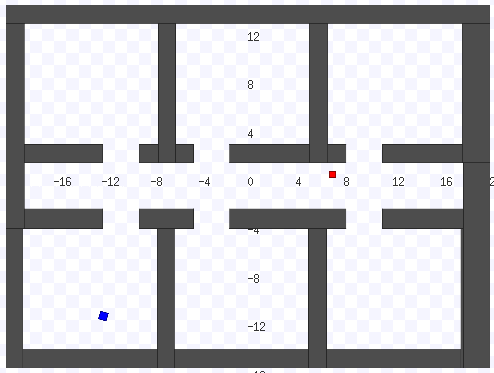
\includegraphics[width=15cm]{Pruebas/simple-rooms-before.png}
			\caption{Posición inicial del robot.}
			\label{begin-sr}	
		\end{figure}
		
		El robot ha avanzado hasta llegar una posición cercana la esquina de la puerta, ha frenado para
		poder girar y bordearla de forma más suave (\ref{turn-b-sr}).
		
		\begin{figure}[H]
			\centering
			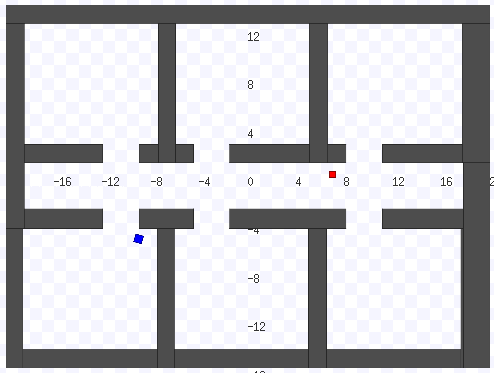
\includegraphics[width=15cm]{Pruebas/simple-rooms-turn-before.png}
			\caption{Posición del robot antes del giro.}
			\label{turn-b-sr}	
		\end{figure}
		
		Ha continuado un poco hacia delante para evitar la pared. Después, ha vuelto a girar para digirse
		hacia su objetivo (\ref{turn-a-sr}).
		
		\begin{figure}[H]
			\centering
			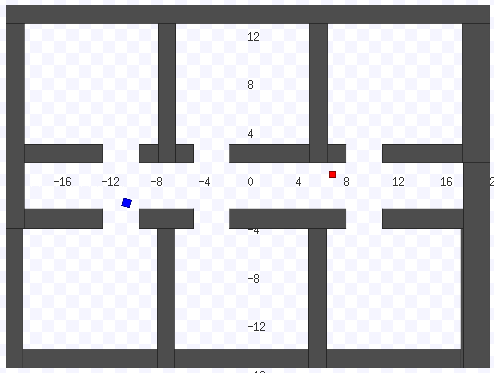
\includegraphics[width=15cm]{Pruebas/simple-rooms-turn-after.png}
			\caption{Posición final del robot después del giro.}
			\label{turn-a-sr}	
		\end{figure}
		
		Finalmente, ha llegado a su objetivo (\ref{end-sr}) y ha aparecido el mensaje de éxito (\ref{res-sr}).

		\begin{figure}[H]
			\centering
			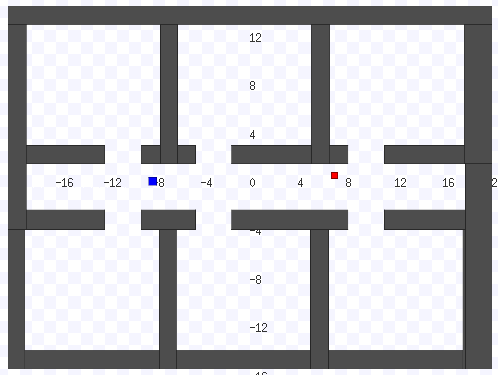
\includegraphics[width=15cm]{Pruebas/simple-rooms-after.png}
			\caption{Posición final del robot.}
			\label{end-sr}	
		\end{figure}

		\begin{figure}[H]
			\centering
			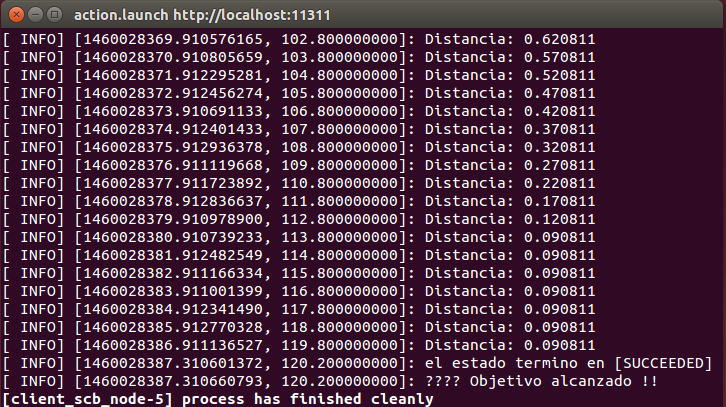
\includegraphics[width=15cm]{Pruebas/simple-rooms-result.png}
			\caption{Resultados del robot.}
			\label{res-sr}	
		\end{figure}
	

	\subsection{Maze\_simple.png}
		Los valores iniciales de este mapa fueron:
		
		\begin{itemize}
			\item \textbf{Posición inicial:} (-2.2, -2.1)
			\item \textbf{Posición objetivo:} (-0.3, -4.1)
		\end{itemize}
		
		La figura \ref{begin-ms} nos muestra el estado inicial.
		
		\begin{figure}[H]
			\centering
			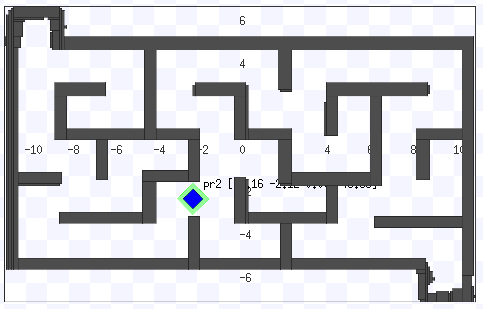
\includegraphics[width=15cm]{Pruebas/maze-simple-before.png}
			\caption{Posición inicial del robot.}
			\label{begin-ms}	
		\end{figure}
		
		Esta prueba, se ha decidido realizarla con un mapa tratado para poder ser usado por \textit{stage}
		y por \textit{rviz}, y así comprobar la compatibilidad de este programa con diversas herramientas
		y que no está limitado al uso de las mismas técnicas.

		Como podemos ver gráficamente en \ref{end-ms} y por terminal en \ref{res-ms}, se consigue alcanzar
		el objetivo.

		\begin{figure}[H]
			\centering
			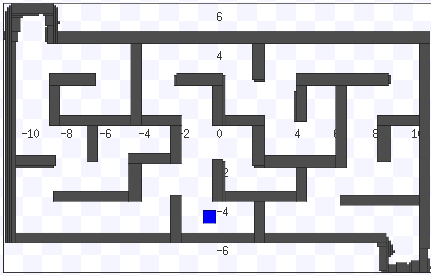
\includegraphics[width=15cm]{Pruebas/maze-simple-after.png}
			\caption{Posición final del robot.}
			\label{end-ms}	
		\end{figure}
		
		\begin{figure}[H]
			\centering
			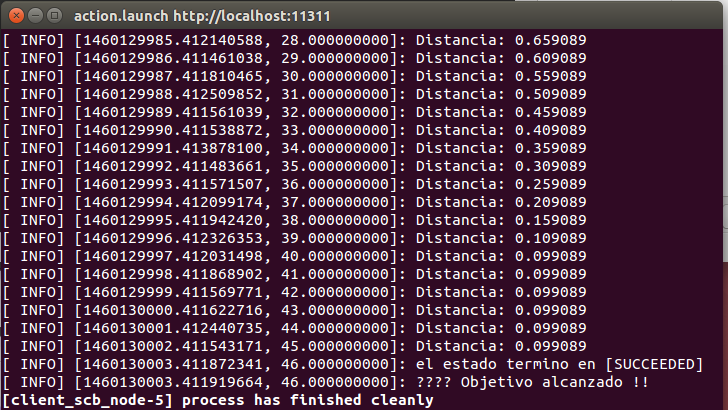
\includegraphics[width=15cm]{Pruebas/maze-simple-result.png}
			\caption{Resultados del robot.}
			\label{res-ms}	
		\end{figure}
		
	
	\subsection{autolab.png}
		En este mapa, la configuración inicial fue:
	
		\begin{itemize}
			\item \textbf{Posición inicial:} (-12, -12)
			\item \textbf{Posición objetivo:} (-12, 12)
		\end{itemize}
		
		Reflejada la figura \ref{begin-a}.
		
		\begin{figure}[H]
			\centering
			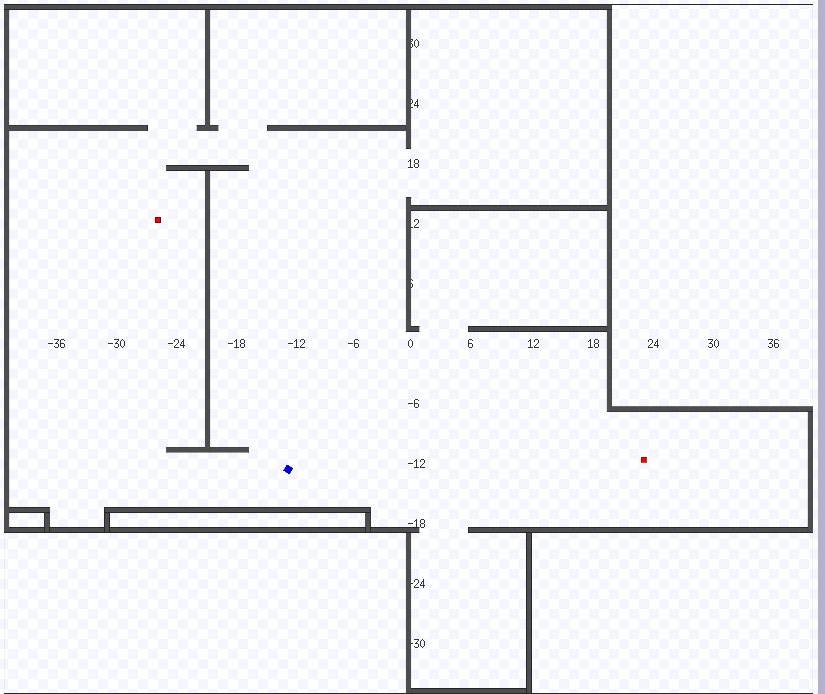
\includegraphics[width=15cm]{Pruebas/autolab-before.png}
			\caption{Posición inicial del robot.}
			\label{begin-a}	
		\end{figure}
		
		En esta prueba, se puede ver que cuando no hay obstáculos cerca el robot, simplemente, describe
		una trayectoria en línea recta para acabar en \ref{end-a}.		
		
		\begin{figure}[H]
			\centering
			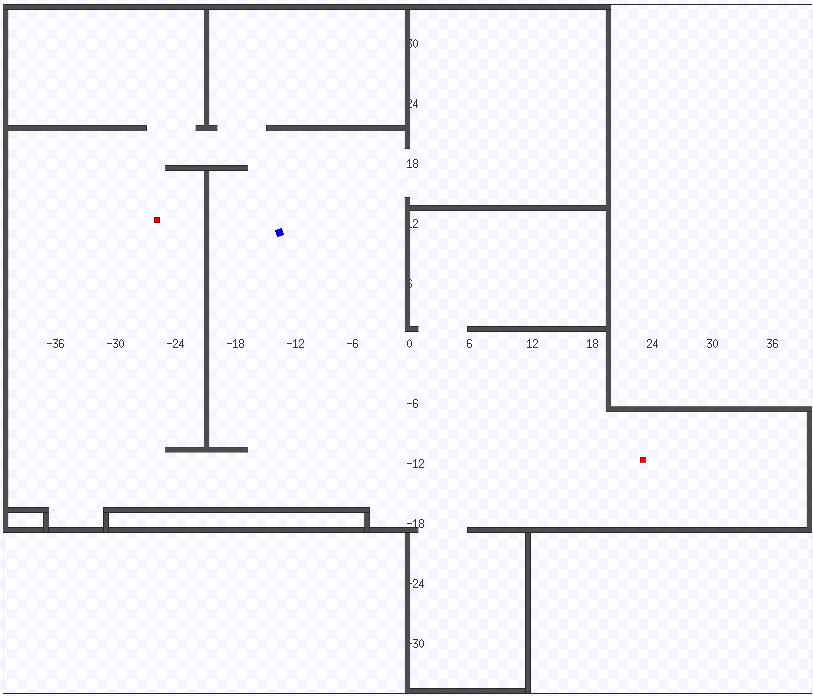
\includegraphics[width=15cm]{Pruebas/autolab-after.png}
			\caption{Posición final del robot.}
			\label{end-a}	
		\end{figure}

\end{document}
